\section{Results}
The results for the on-lattice simulations can be found in figure \ref{fig:2d-DLA_400}. \textcolor{red}{??? The fractal dimension was calculated straight forward in this case, only looking at the relation between $R$ and $N$, not using equation \eqref{eq:N_Rg_rel}. Should probalby also update the figure with a figure of more particles, so just get it done some weekend. Should probably also fix the calculation of $d_f$.} It is worth noting that the fractal dimension oobtained from \ref{fig:2d-DLA_400} is in accordance with what was found in \cite{PhysRevLett.47.1400}, although the method of calculation was slightly different so an exact accordance is not to be expected. 

\begin{figure}[h]
	\begin{center}
		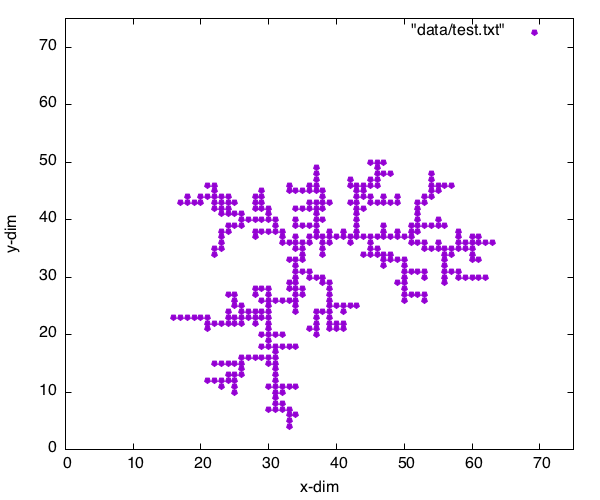
\includegraphics[width = 0.8\textwidth]{fig/on_lattice_400_p_75_g.png}
		\caption{\textcolor{red}{??? I'm sure there could be some improvements to this.} On-lattice DLA simulation of 400 particles on a 75 by 75 grid.  This particular cluster has a fractal dimension of $d_f = 1.70999$.}
		\label{fig:2d-DLA_400}
	\end{center}
\end{figure}

The results for the off-lattice simulations can be found in figure \ref{fig:2d-DLA_1mill}, with corresponding regression plot in figure \ref{fig:loglog2d-DLA_1mill} (see equation \eqref{eq:N_Rg_rel}). These results fits with the results obtained by Kuijpers \cite{Kuijpers2014841}.
\begin{figure}
	\begin{center}
		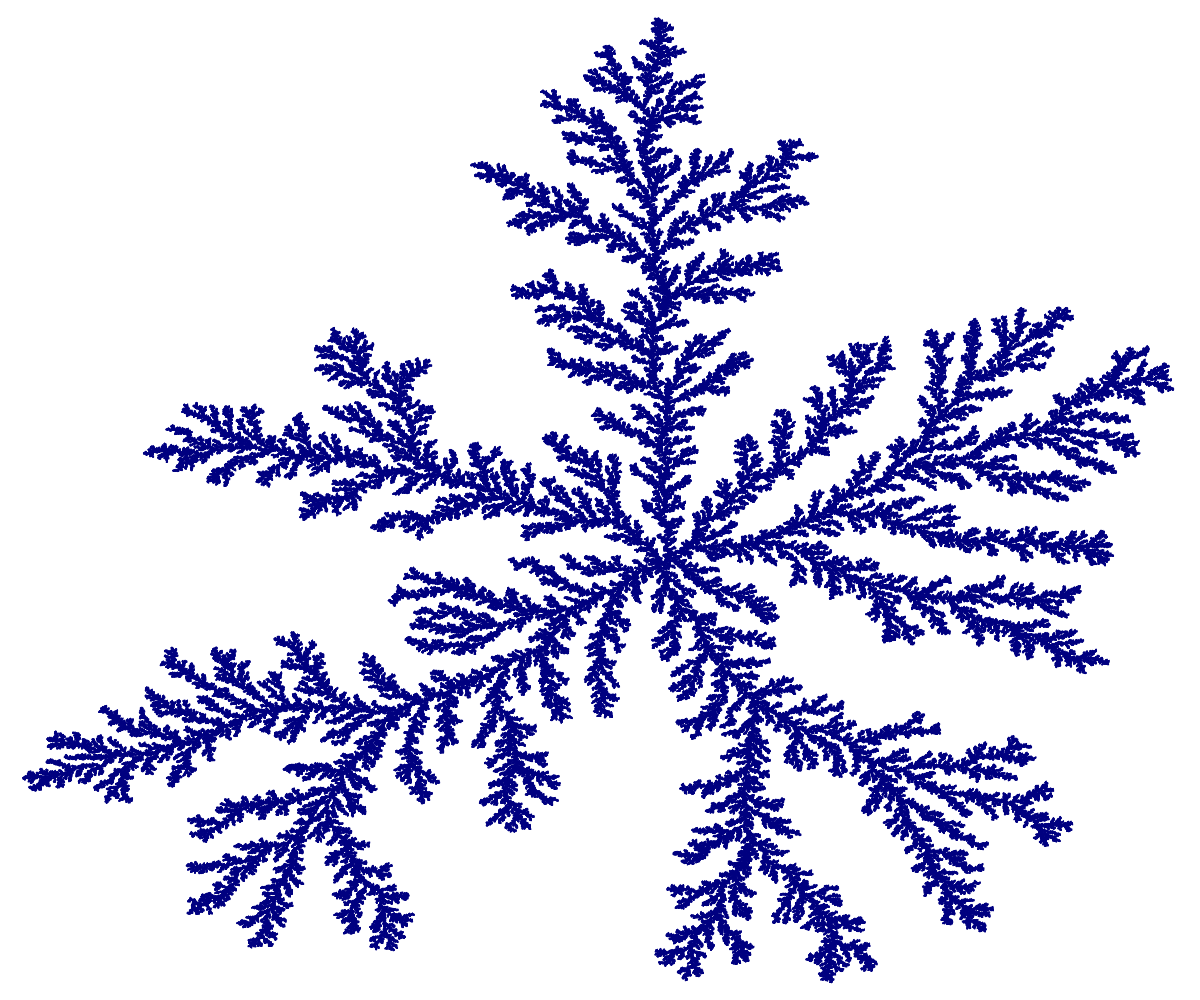
\includegraphics[width = 0.8\textwidth]{fig/1_(1_7248).png}
		\caption{\textcolor{red}{??? Replace with a borderless version, so that one doesn't have to have x-ticks and x-labels etc...} Off-lattice DLA simulation of $10^6$ particles. This particular cluster has a fractal dimension of $d_f = 1.7248 \pm 0.006033$.}
		\label{fig:2d-DLA_1mill}
	\end{center}
\end{figure}

\begin{figure}
	\begin{center}
		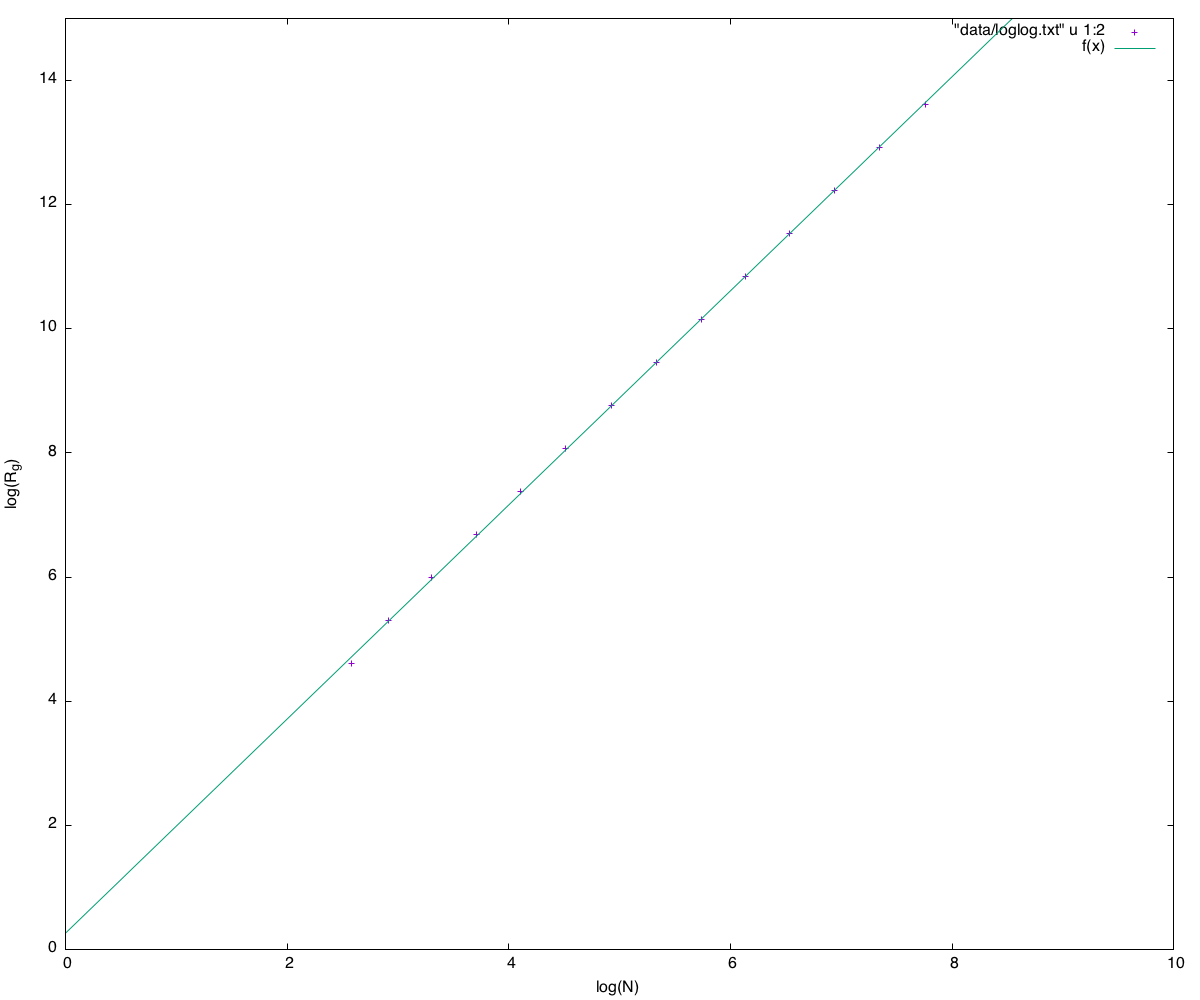
\includegraphics[width = 0.8\textwidth]{fig/loglog(1_7248).png}
		\caption{The log-log plot of $N$ and $R_g$. From this, the fractal dimension was calculated using linear regression.  \textcolor{red}{??? replace with a plot including the slope/linear approximation.}}
		\label{fig:loglog2d-DLA_1mill}
	\end{center}
\end{figure}




\begin{figure}[h]
	\begin{center}
		\begin{subfigure}[t]{0.45\textwidth}
			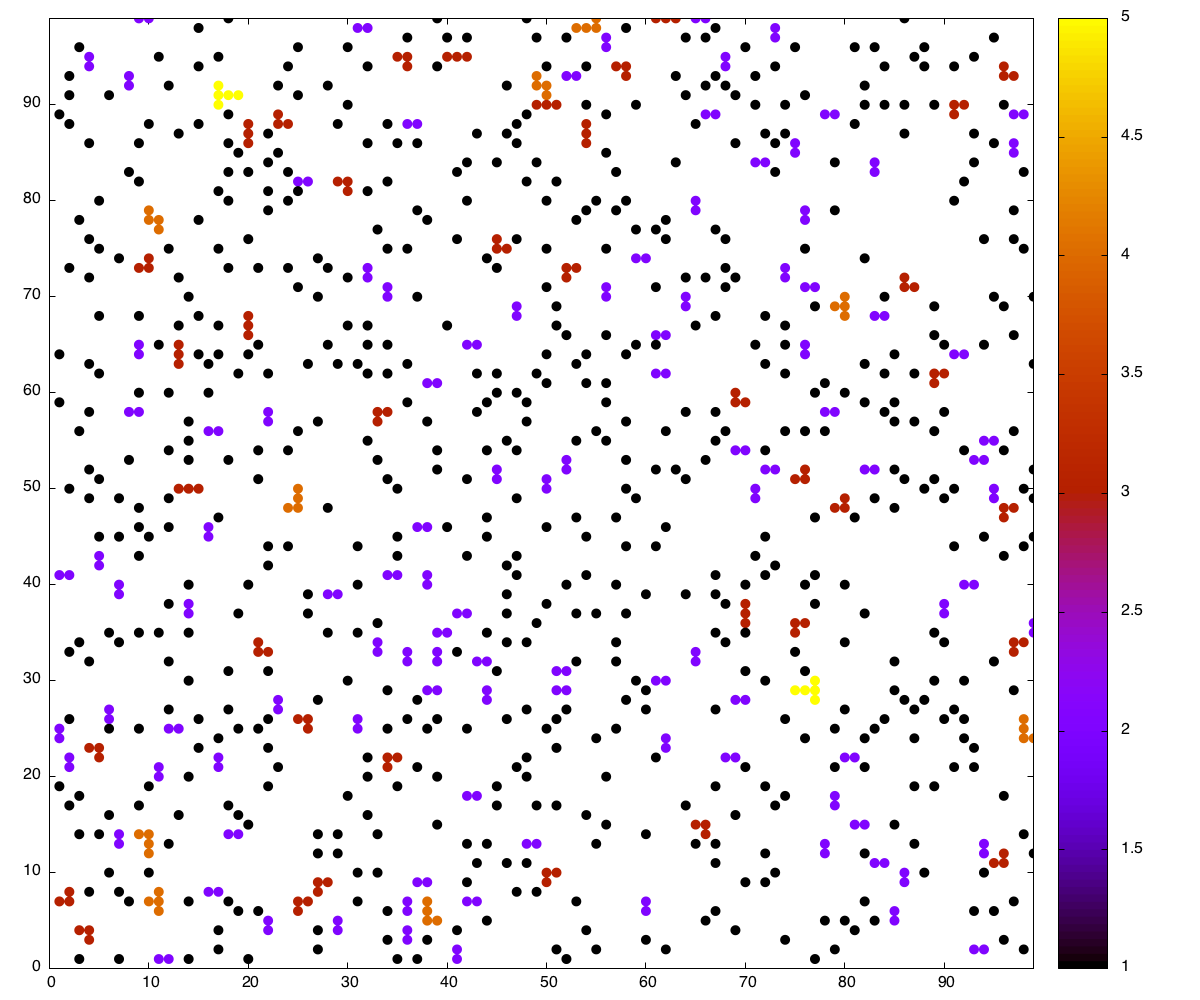
\includegraphics[width = \textwidth]{fig/000_on.png}
			\caption{How the domain looks after $ t = 0 $ \textcolor{red}{??? Change!}}
			\label{fig:0}
		\end{subfigure}
		\begin{subfigure}[t]{0.45\textwidth}
			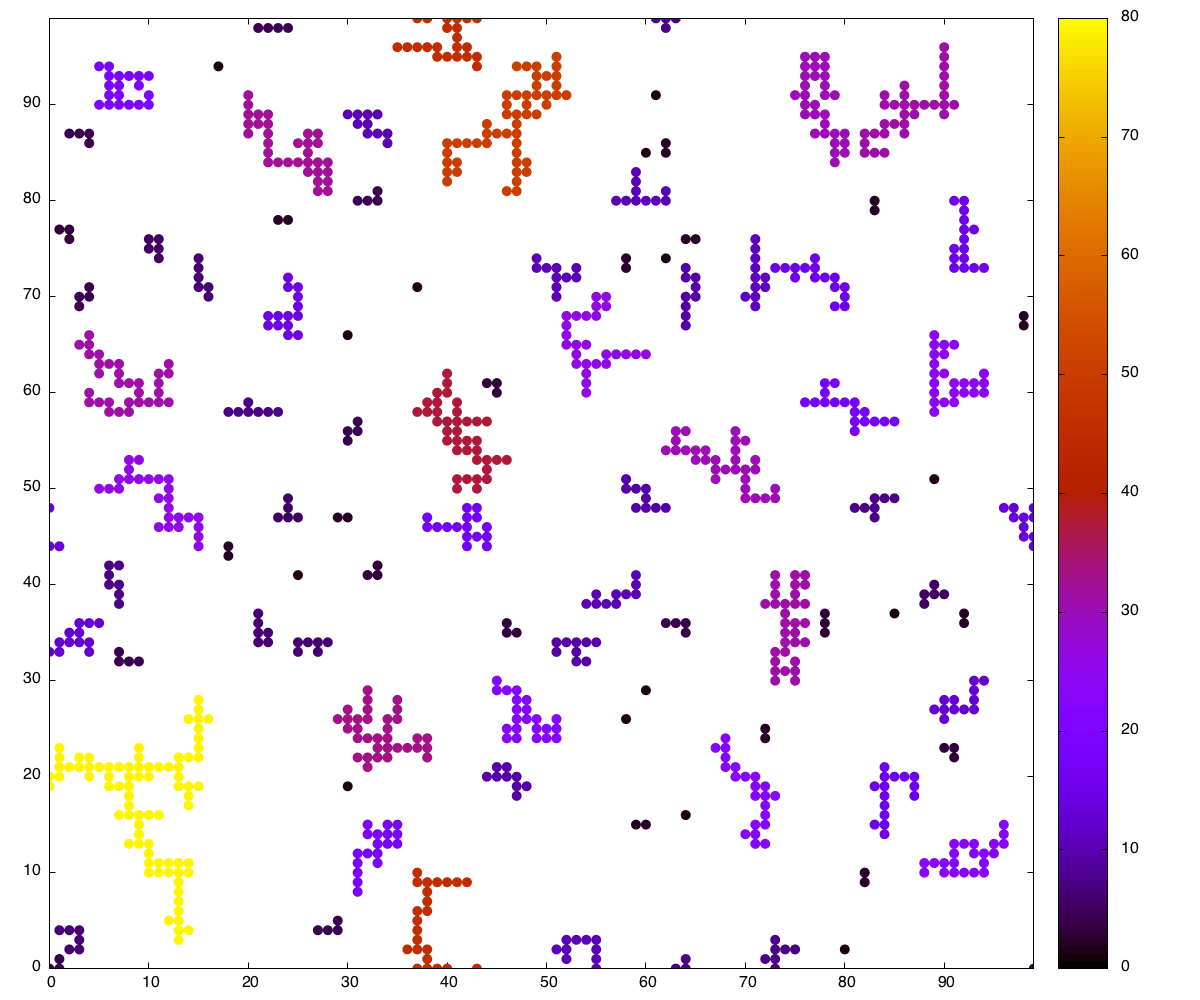
\includegraphics[width = \textwidth]{fig/0033_on.png}
			\caption{How the domain looks after $ t = 33 $ \textcolor{red}{??? Change!} }
			\label{fig:33}
		\end{subfigure}
		\begin{subfigure}[t]{0.45\textwidth}
		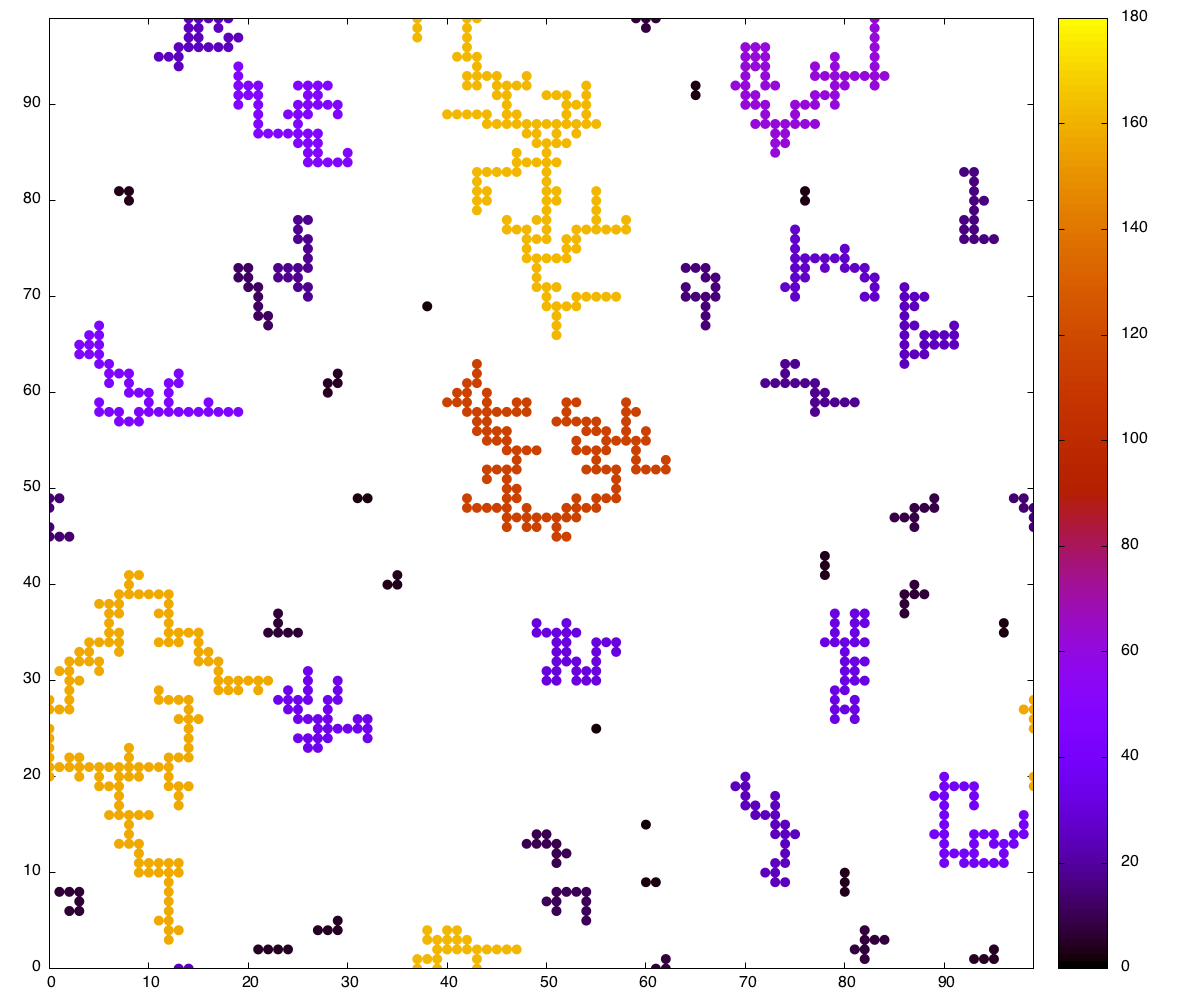
\includegraphics[width = \textwidth]{fig/0067_on.png}
			\caption{How the domain looks after $ t = 67 $ \textcolor{red}{??? Change!}}
			\label{fig:67}
		\end{subfigure}
		\begin{subfigure}[t]{0.45\textwidth}
			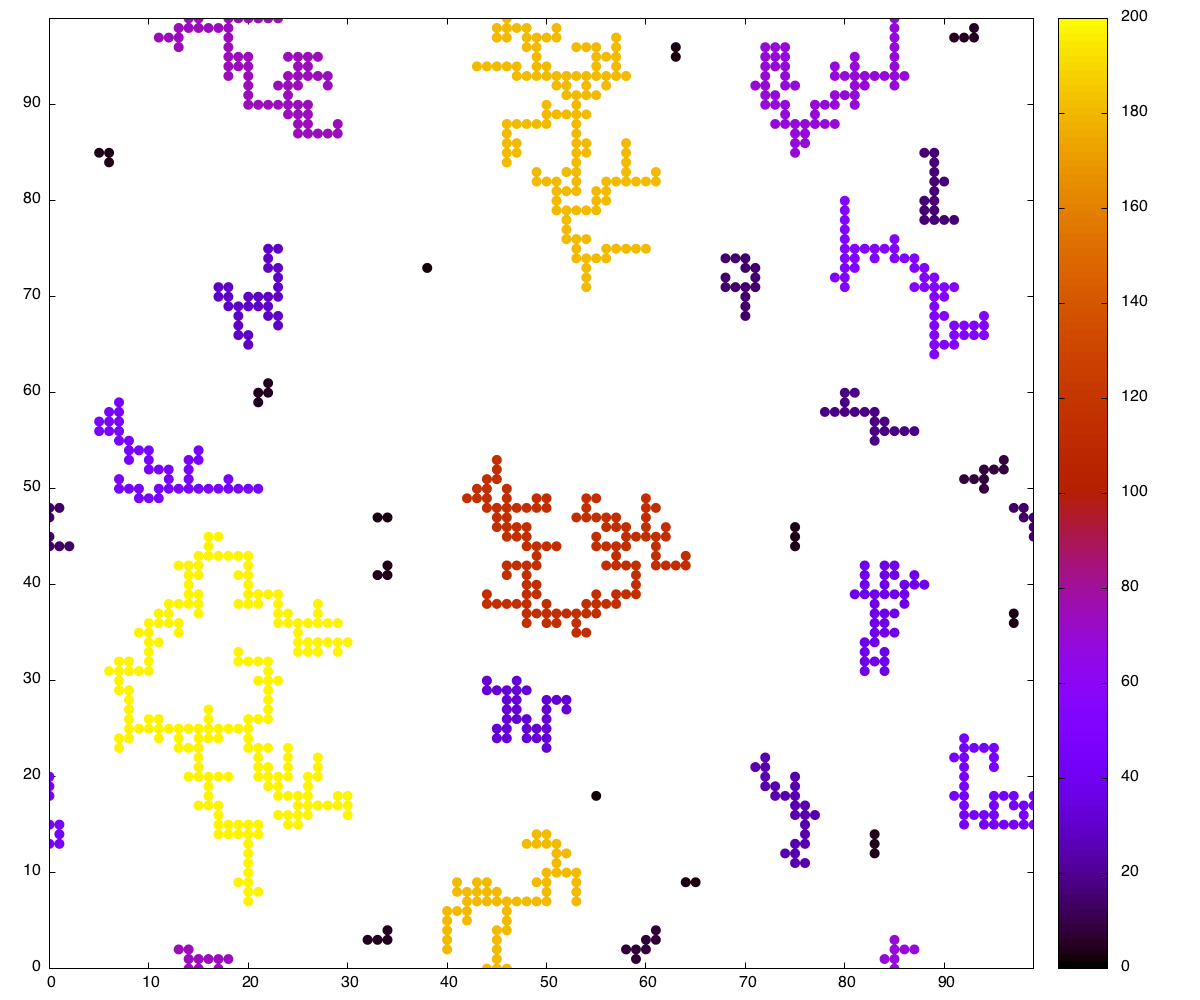
\includegraphics[width = \textwidth]{fig/0099_on.png}
			\caption{After time $t = 100$ \textcolor{red}{or whatever, must be changed at some point.}}
			\label{fig:100}
		\end{subfigure}
		\caption{Sequence of how the aggregation process might look on grid. \textcolor{red}{??? has to be changed!}}
		\label{fig:arrays}
	\end{center}
\end{figure}


\begin{figure}[h]
	\begin{center}
		\begin{subfigure}[t]{0.45\textwidth}
			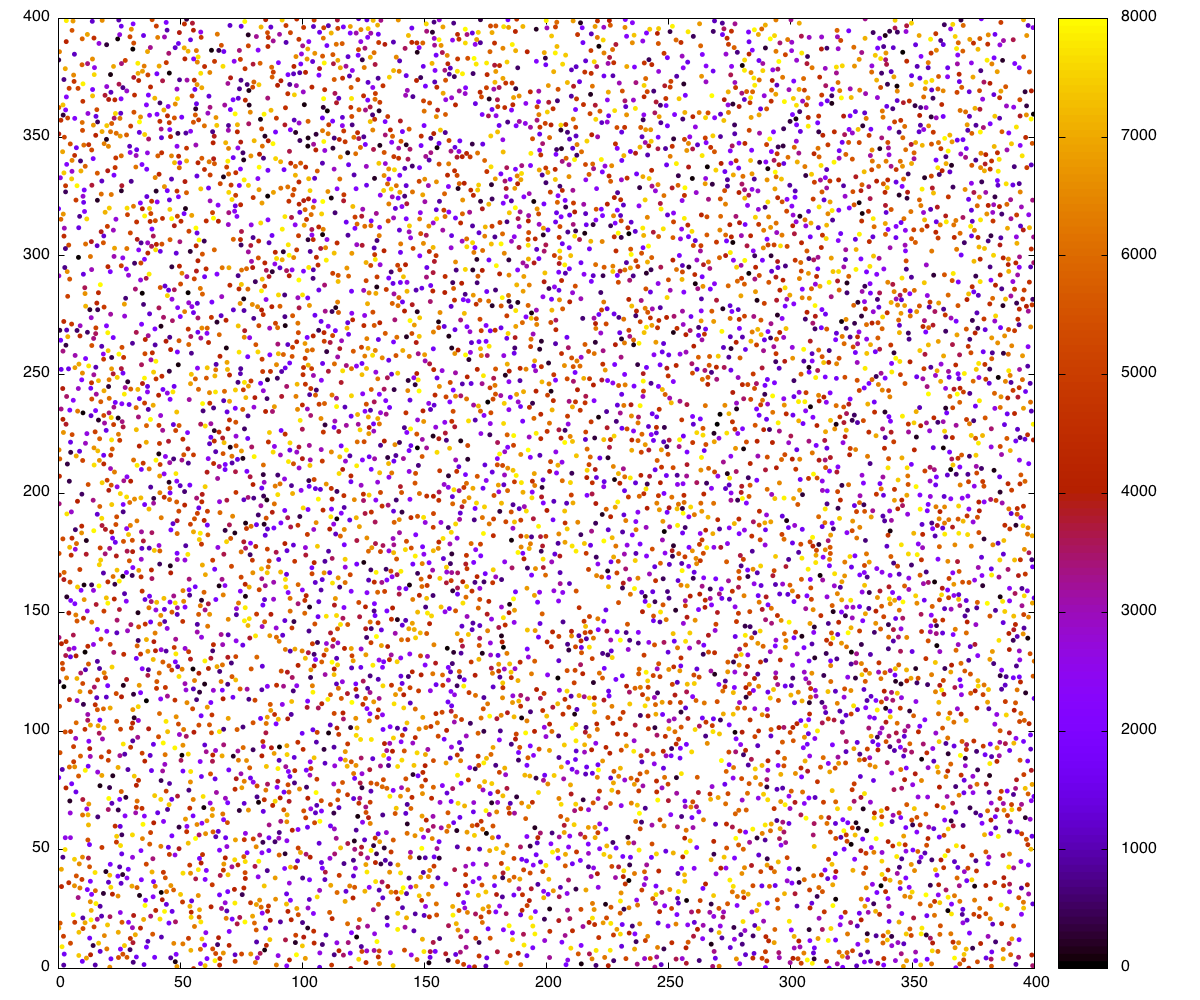
\includegraphics[width = \textwidth]{fig/000_off.png}
			\caption{How the domain looks after $ t = 0.00 s $ \textcolor{red}{??? Change!}}
			\label{fig:0}
		\end{subfigure}
		\begin{subfigure}[t]{0.45\textwidth}
			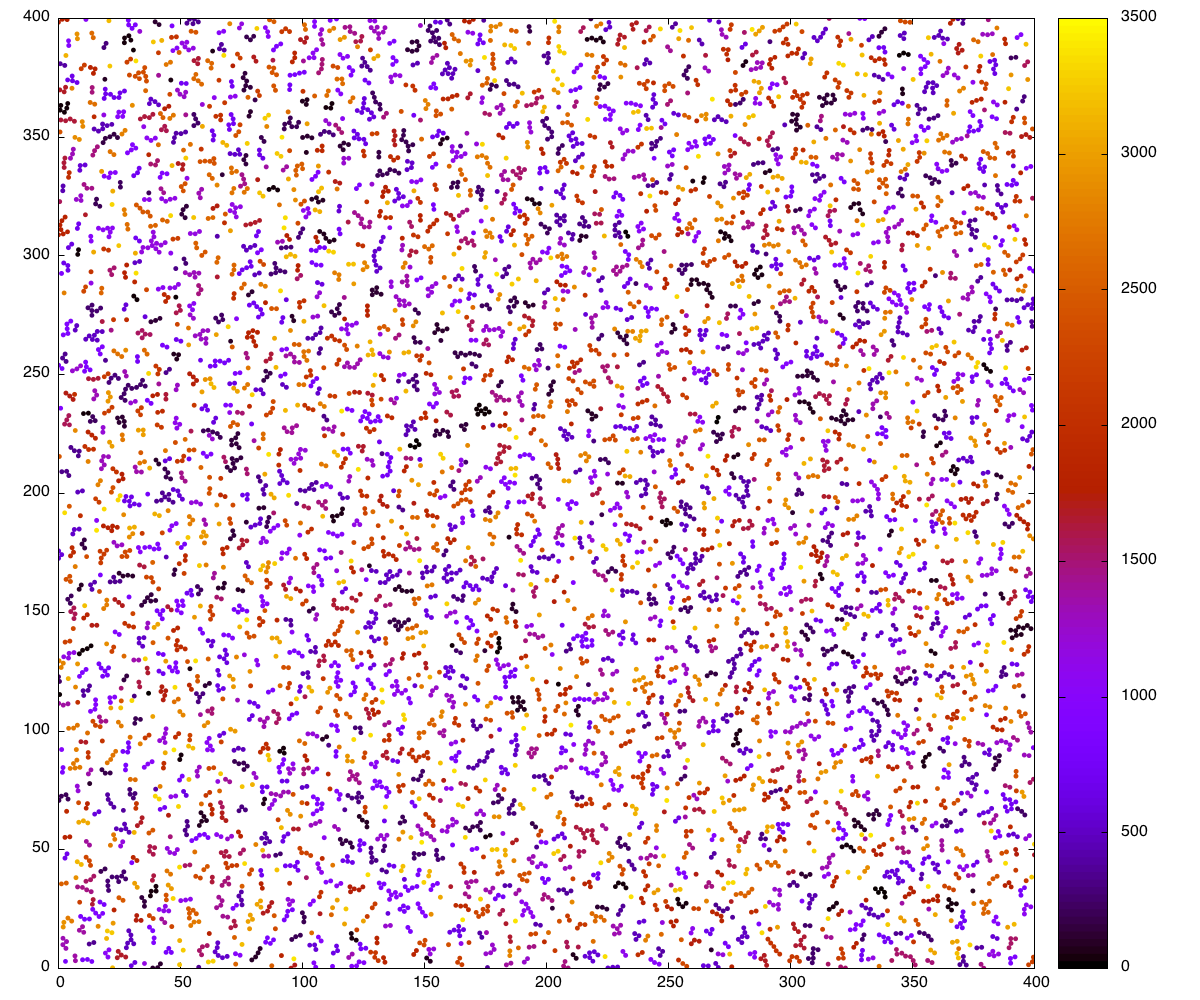
\includegraphics[width = \textwidth]{fig/0010_off.png}
			\caption{How the domain looks after $ t = 0.10s $ \textcolor{red}{??? Change!} }
			\label{fig:33}
		\end{subfigure}
		\begin{subfigure}[t]{0.45\textwidth}
		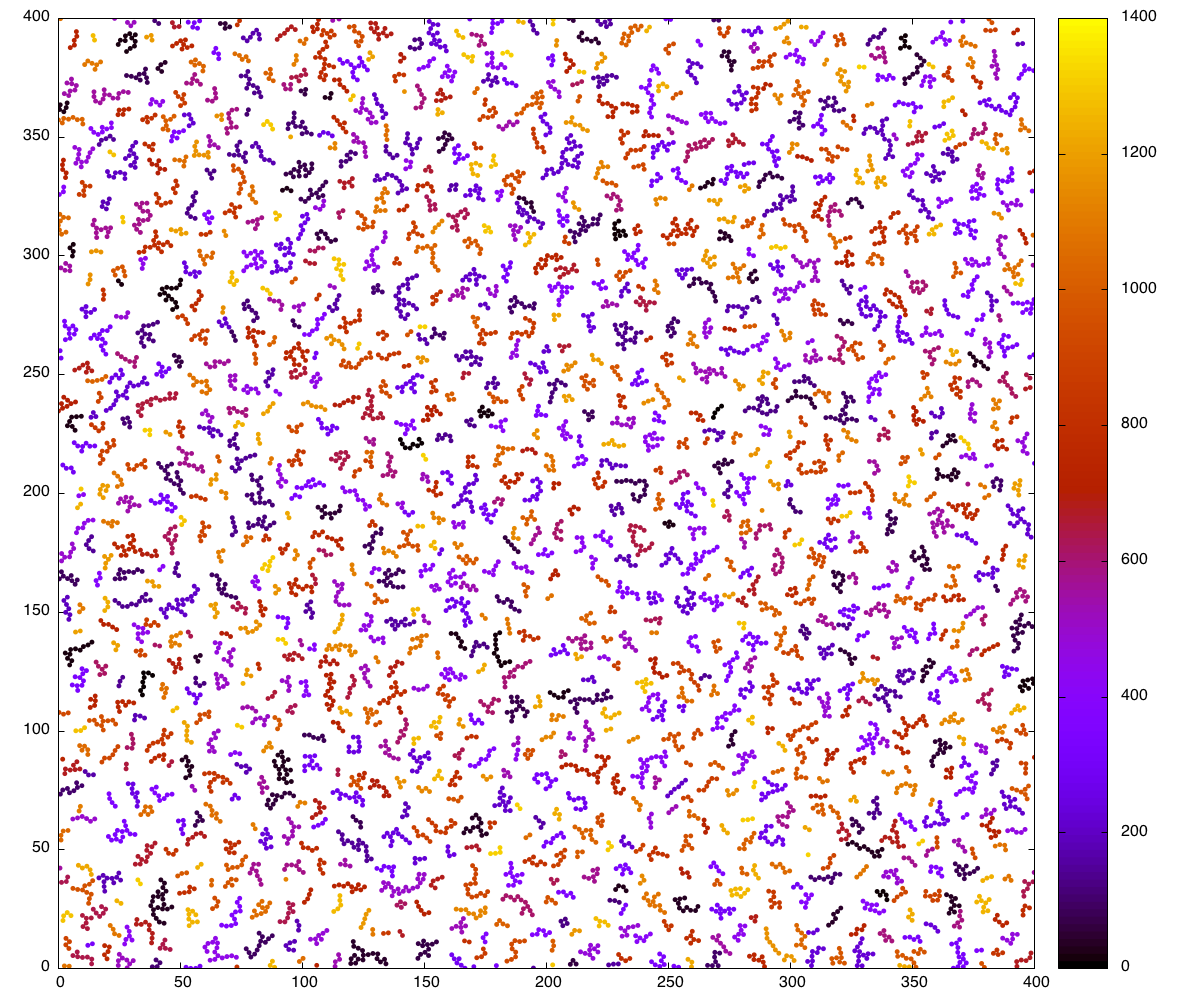
\includegraphics[width = \textwidth]{fig/00100_off.png}
			\caption{How the domain looks after $ t = 1.00 s $ \textcolor{red}{??? Change!}}
			\label{fig:67}
		\end{subfigure}
		\begin{subfigure}[t]{0.45\textwidth}
			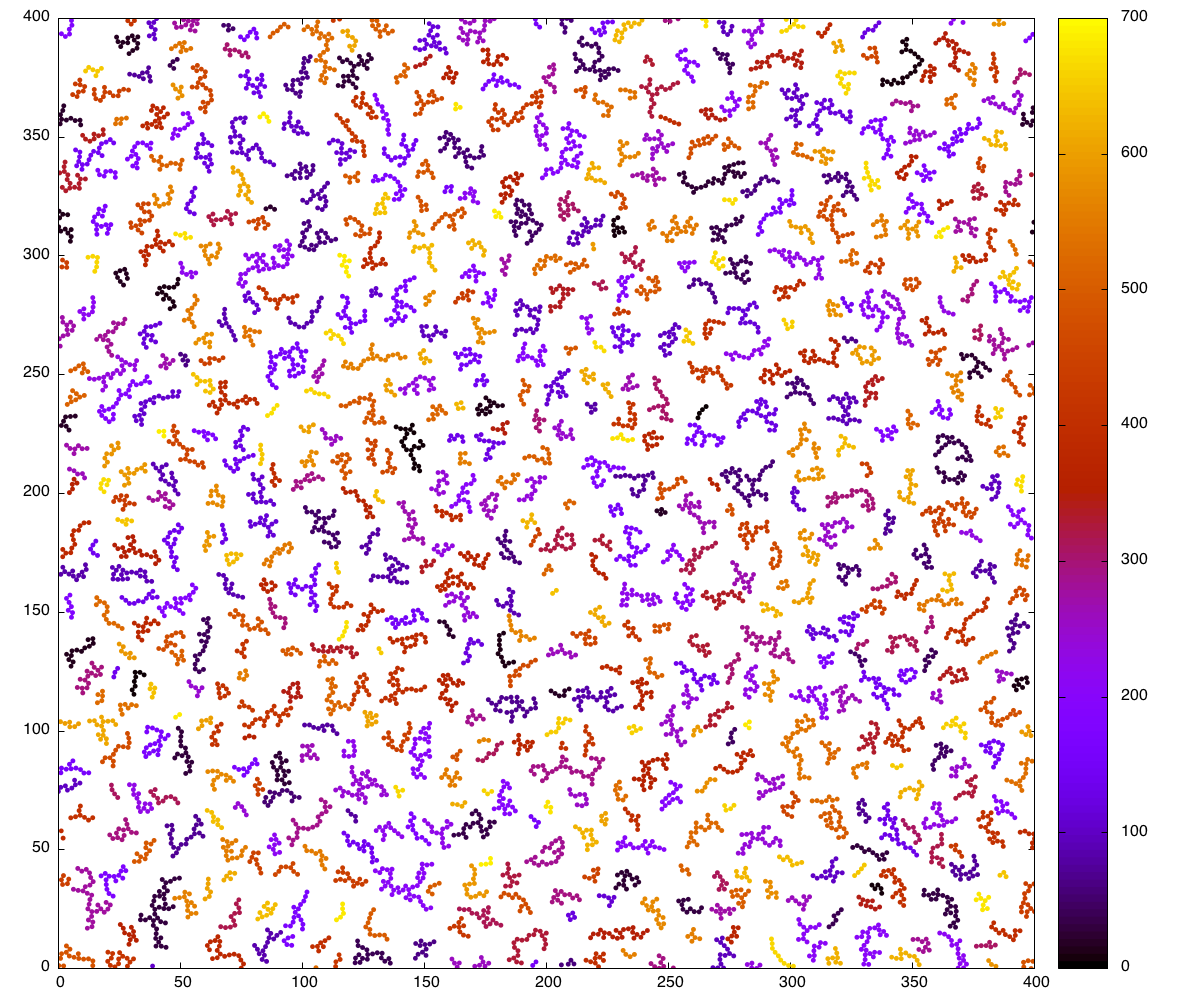
\includegraphics[width = \textwidth]{fig/00500_off.png}
			\caption{After time $t = 5.00 s$ \textcolor{red}{or whatever, must be changed at some point.}}
			\label{fig:100}
		\end{subfigure}
		\caption{Sequence of how the aggregation process might look on grid. This configuration was 8000 particles on a $400 \times 400$ grid, meaning $\rho = 0.05$. This was done using steps of $dt = 0.01$, and as one would expect, the agglomeration of larger clusters is a very slow process. \textcolor{red}{??? has to be changed!}}
		\label{fig:arrays}
	\end{center}
\end{figure}



\begin{figure}
	\begin{center}
		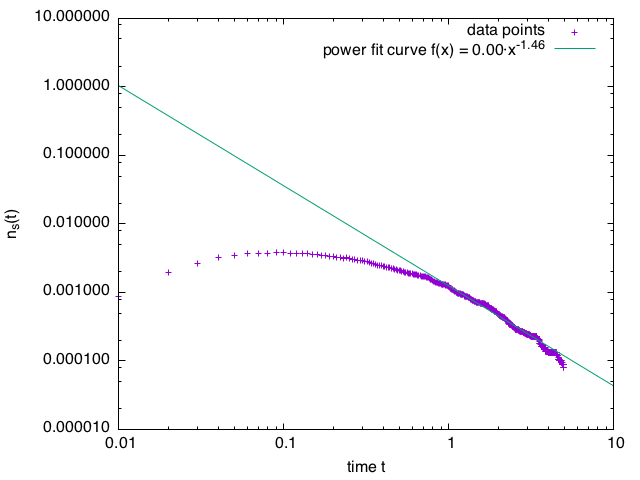
\includegraphics[width = 0.8\textwidth]{fig/plotTest.png}
		\caption{\textcolor{red}{??? temporary: The log-log plot of the time evolution of $n_s(t)$ for a cluster of size $s = 10$. The slope approximation to the data yields $w \approx 1.46$.}}
		\label{fig:loglog2d-DLA_1mill}
	\end{center}
\end{figure}